%% Based on a TeXnicCenter-Template by Gyorgy SZEIDL.
%%%%%%%%%%%%%%%%%%%%%%%%%%%%%%%%%%%%%%%%%%%%%%%%%%%%%%%%%%%%%

%------------------------------------------------------------
%
\documentclass{article}%
%Options -- Point size:  10pt (default), 11pt, 12pt
%        -- Paper size:  letterpaper (default), a4paper, a5paper, b5paper
%                        legalpaper, executivepaper
%        -- Orientation  (portrait is the default)
%                        landscape
%        -- Print size:  oneside (default), twoside
%        -- Quality      final(default), draft
%        -- Title page   notitlepage, titlepage(default)
%        -- Columns      onecolumn(default), twocolumn
%        -- Equation numbering (equation numbers on the right is the default)
%                        leqno
%        -- Displayed equations (centered is the default)
%                        fleqn (equations start at the same distance from the right side)
%        -- Open bibliography style (closed is the default)
%                        openbib
% For instance the command
%           \documentclass[a4paper,12pt,leqno]{article}
% ensures that the paper size is a4, the fonts are typeset at the size 12p
% and the equation numbers are on the left side
%
\usepackage{amsmath}%
\usepackage{amsfonts}%
\usepackage{amssymb}%
\usepackage{graphicx}
\usepackage{subfigure}
%-------------------------------------------
\newtheorem{theorem}{Theorem}
\newtheorem{acknowledgement}[theorem]{Acknowledgement}
\newtheorem{algorithm}[theorem]{Algorithm}
\newtheorem{axiom}[theorem]{Axiom}
\newtheorem{case}[theorem]{Case}
\newtheorem{claim}[theorem]{Claim}
\newtheorem{conclusion}[theorem]{Conclusion}
\newtheorem{condition}[theorem]{Condition}
\newtheorem{conjecture}[theorem]{Conjecture}
\newtheorem{corollary}[theorem]{Corollary}
\newtheorem{criterion}[theorem]{Criterion}
\newtheorem{definition}[theorem]{Definition}
\newtheorem{example}[theorem]{Example}
\newtheorem{exercise}[theorem]{Exercise}
\newtheorem{lemma}[theorem]{Lemma}
\newtheorem{notation}[theorem]{Notation}
\newtheorem{problem}[theorem]{Problem}
\newtheorem{proposition}[theorem]{Proposition}
\newtheorem{remark}[theorem]{Remark}
\newtheorem{solution}[theorem]{Solution}
\newtheorem{summary}[theorem]{Summary}
\newenvironment{proof}[1][Proof]{\textbf{#1.} }{\ \rule{0.5em}{0.5em}}

\begin{document}

\begin{flushleft}
\textbf{Course:} CSC522, Automated Learning and Data Analysis\\
\textbf{Homework 2}\\
\textbf{Student: Xusheng Xiao}\\
\textbf{Unity ID: xxiao2} \\
\textbf{Email: xxiao2@ncsu.edu}
\end{flushleft}

\noindent{\hrulefill}

\bigskip

\begin{enumerate}
	\item (15 points) Use k-means on the non-noise data by setting k=2,3,4,5,6,7,8,9,10. For each value of k, compute the SSE (sum of squared error) of clustering result, and the average silhouette of clustering result. Plot the SSE curve and silhouette curve w.r.t the various k values. (You can use any kind of distance measure.)
	\begin{table}[h]
	\begin{tabular}{|p{2cm}|c|c|c|c|c|c|c|c|c|}
	    \hline
		Evaluation Measure&\multicolumn{9}{|c|}{Value of k (Size of Cluster)}\\ \cline{2-10}
		& 2 &3 &4 &5 &6 &7 &8 &9 &10 \\ \hline
		SSE (Euclidean Distance) & 104260 & 61018 &48231 &37211 &29493 &20158 &18151 &16882 &13018 \\ \hline
		Average Silhouette & 0.6735 & 0.6860 &0.6272 &0.6494 &0.6487 &0.7227 &0.7144 &0.6999 &0.7415\\ \hline
		
	\end{tabular}
	\caption{k-means for non-noise data}
	\end{table}
	
	Figure \ref{fig:kmeans-non-noisy-sse} shows the SSE curve and Figure \ref{fig:kmeans-non-noisy-avgsil} shows the average silhouette curve.
	%\usepackage{graphics} is needed for \includegraphics
	%\usepackage{graphics} is needed for \includegraphics
\begin{figure}[h]
	\centering
 	 \subfigure[SSE (Euclidean Distance) of kmeans on non-noisy data]{
		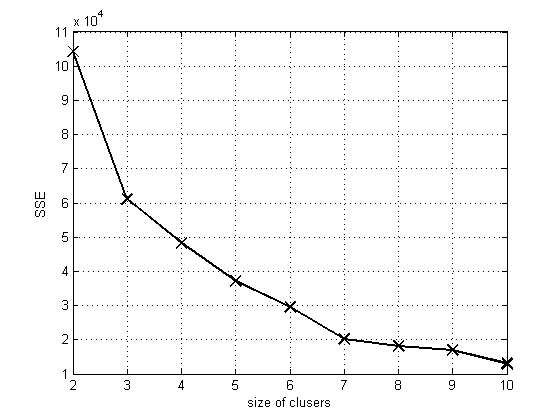
\includegraphics[scale=0.385]{fig/kmeans-data-sse.png}
	    \label{fig:kmeans-non-noisy-sse}
	}
	\subfigure[Average Silhouette of kmeans on non-noisy data]{
		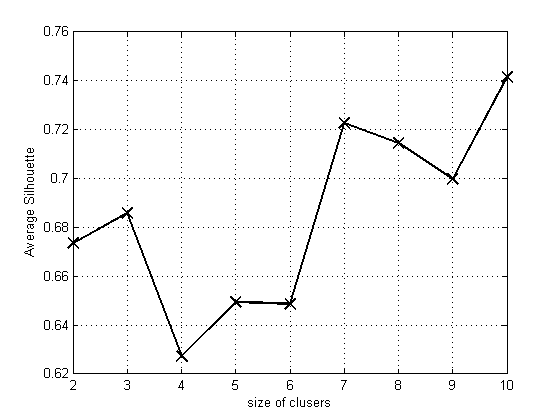
\includegraphics[scale=0.385]{fig/kmeans-data-sil.png}
   		 \label{fig:kmeans-non-noisy-avgsil}
	}
	\caption{Kmeans on non-noisy data}
\end{figure}
	
% \begin{figure}[!iht]
% \begin{center}
%   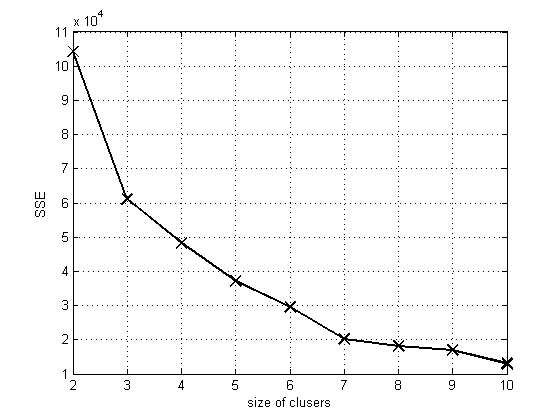
\includegraphics[scale=0.65]{fig/kmeans-data-sse.png}
%   \caption{SSE (Euclidean Distance) of kmeans on non-noisy data}
%   \label{fig:kmeans-non-noisy-sse}
% \end{center}
% \end{figure}
% 
% \begin{figure}[!iht]
% \begin{center}
%   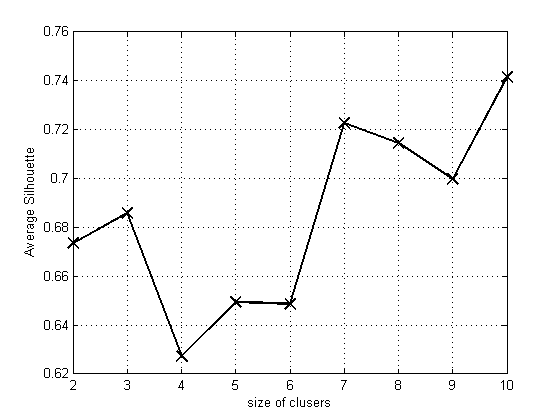
\includegraphics[scale=0.65]{fig/kmeans-data-sil.png}
%   \caption{Average Silhouette of kmeans on non-noisy data}
%   \label{fig:kmeans-non-noisy-avgsil}
% \end{center}
% \end{figure}
	
	\item (15 points) Use k-means on the noisy data by setting k=2,3,4,5,6,7,8,9,10. For each value of k, compute the SSE of clustering result, and the average silhouette of clustering result. Plot the SSE curve and silhouette curve w.r.t the various k values.
	\begin{table}[h]
	\begin{tabular}{|p{2cm}|c|c|c|c|c|c|c|c|c|}
	    \hline
		Evaluation Measure&\multicolumn{9}{|c|}{Value of k (Size of Cluster)}\\ \cline{2-10}
		& 2 &3 &4 &5 &6 &7 &8 &9 &10 \\ \hline
		SSE (Euclidean Distance) & 110750 & 66625 &51930 &39924 &29435 &22158 &20113 &16816 &14732 \\ \hline
		Average Silhouette & 0.6710 & 0.6756 &0.6147 &0.6531 &0.6743 &0.7140 &0.6907 &0.6871 &0.6908\\ \hline
		
	\end{tabular}
	\caption{k-means for noisy data}
	\end{table}
	
	Figure \ref{fig:kmeans-noisy-sse} shows the SSE curve and Figure \ref{fig:kmeans-noisy-avgsil} shows the average silhouette curve.

\begin{figure}[h]
	\centering
 	 \subfigure[SSE (Euclidean Distance) of kmeans on noisy data]{
		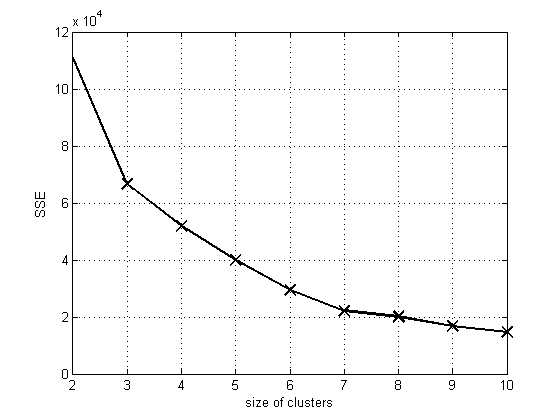
\includegraphics[scale=0.385]{fig/kmeans-noisy-data-sse.png}
	    \label{fig:kmeans-noisy-sse}
	}
	\subfigure[Average Silhouette of kmeans on noisy data]{
		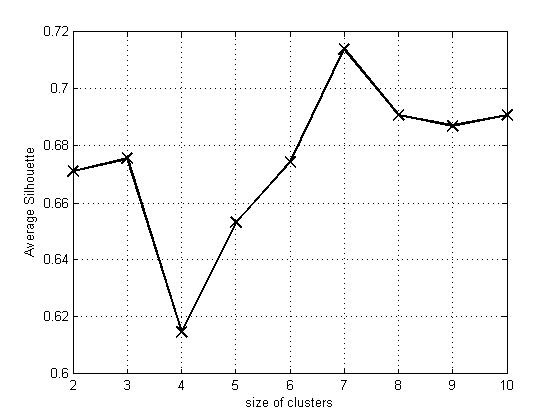
\includegraphics[scale=0.385]{fig/kmeans-noisy-data-sil.png}
	    \label{fig:kmeans-noisy-avgsil}
	}
	\caption{Kmeans on noisy data}
\end{figure}
	
% 	\begin{figure}[!iht]
% \begin{center}
%   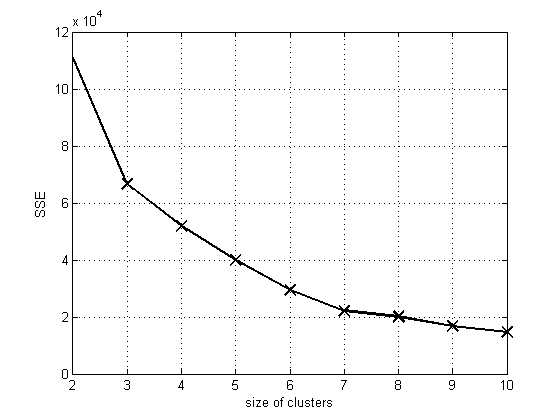
\includegraphics[scale=0.65]{fig/kmeans-noisy-data-sse.png}
%   \caption{SSE (Euclidean Distance) of kmeans on noisy data}
%   \label{fig:kmeans-noisy-sse}
% \end{center}
% \end{figure}
% 
% \begin{figure}[!iht]
% \begin{center}
%   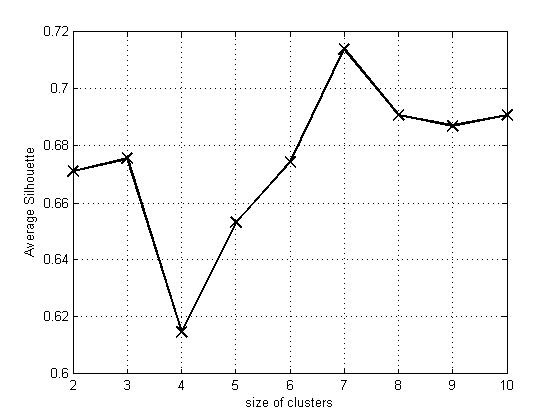
\includegraphics[scale=0.65]{fig/kmeans-noisy-data-sil.png}
%   \caption{Average Silhouette of kmeans on noisy data}
%   \label{fig:kmeans-noisy-avgsil}
% \end{center}
% \end{figure}	
	
	\item (5 points) Can you tell the �correct� number of clusters from the SSE curve and silhouette curve? What is the correct number?
	
	\textbf{Answer:} The ``correct'' number of clusters should be 10. When the number of clusters is 10, the SSE is the lowest value and the average silhouette is close to 1.
	
	\item (15 points) Use agglomerative hierarchical clustering method on the non-noise data. Try 4 different setting of linkage,
		\begin{itemize}
  			\item single (min, shortest)
			\item complete (max, furthest)
			\item average (average distance)			
			\item ward (inner squared distance, minimum variance algorithm)
		\end{itemize}
		Compute the �Cophenetic correlation coefficient� for each clustering result with different setting of linkage. Make a table to show the 4 Cophenetic correlation coefficients and tell which one is the best.
		
		\begin{table}[h]
		\centering
	\begin{tabular}{|p{2cm}|c|c|c|c|c|}
	    \hline
		Evaluation Measure&\multicolumn{4}{|c|}{Setting of linkage}\\ \cline{2-5}
		& single & complete & average & ward  \\ \hline
		Cophenetic correlation coefficient & 0.6618 & 0.7734 &0.7780 &0.7461  \\ \hline
		
	\end{tabular}
	\caption{Agglomerative hierarchical clustering for non-noisy data}
	\end{table}
	
	The average linkage is the best, since its value 0.7780 is the highest.
		
	\item (15 points) Use agglomerative hierarchical clustering method on the noisy data. Try 4 different setting of linkage,
		\begin{itemize}
  			\item single (min, shortest)
			\item complete (max, furthest)
			\item average (average distance)			
			\item ward (inner squared distance, minimum variance algorithm)
		\end{itemize}
		Compute the �Cophenetic correlation coefficient� for each clustering result with different setting of linkage. Make a table to show the 6 Cophenetic correlation coefficients and tell which one is the best.
		
		\begin{table}[h]
		\centering
	\begin{tabular}{|p{2cm}|c|c|c|c|c|}
	    \hline
		Evaluation Measure&\multicolumn{4}{|c|}{Setting of linkage}\\ \cline{2-5}
		& single & complete & average & ward  \\ \hline
		Cophenetic correlation coefficient & 0.6549 & 0.7214 &0.7703 &0.7361  \\ \hline
	\end{tabular}
	\caption{Agglomerative hierarchical clustering for noisy data}
	\end{table}
	
	The average linkage is the best, since its value 0.7703 is the highest.
		
	\item (5 points) Are the best settings of linkage in Question 4 and Question 5 the same? If they are not the same, why ?
	
	\textbf{Answer:} Both the best settings for non-noisy and noisy data are average links. 
	
	\item (15 points) DbScan on the non-noise data. Try different settings of parameter Minpts and Eps. Plot the best clustering result you think (using different colors to show different clusters) and answer:
		\begin{itemize}
  			\item How the clustering result is changing when you increase Minpts ?
  			
  			\textbf{Answer:} The number of clusters decreases.
  			
			\item How the clustering result is changing when you increase Eps ?
			
			\textbf{Answer:} The number of clusters increases.
			
		\end{itemize}
		
		When the Minpts = 14 and Eps = 1.6, the clustering result looks pretty good. Figure \ref{fig:non-noisy-data} shows the plot of non-noisy data and Figure \ref{fig:dbscan-non-noisy-data} shows the clustering result using DBScan.
		
		\begin{figure}[!iht]
		\centering
 		 \subfigure[Non-noisy data]{
			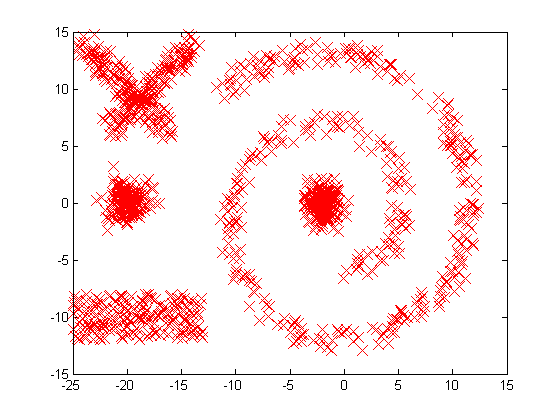
\includegraphics[scale=0.5]{fig/data.png}
		    \label{fig:non-noisy-data}
		}
		\subfigure[DBScan on noisy data where Minpts = 14 and Eps = 1.6]{
			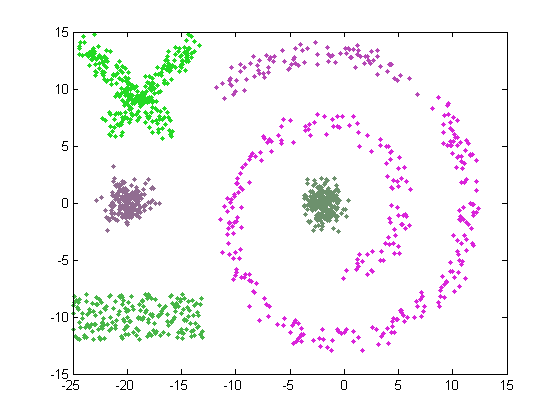
\includegraphics[scale=0.5]{fig/dbscan-non-noisy-data.png}
	    	\label{fig:dbscan-non-noisy-data}
		}
		\caption{DBScan on non-noisy data}
		\end{figure}
		
% \begin{figure}[!iht]
% \begin{center}
%   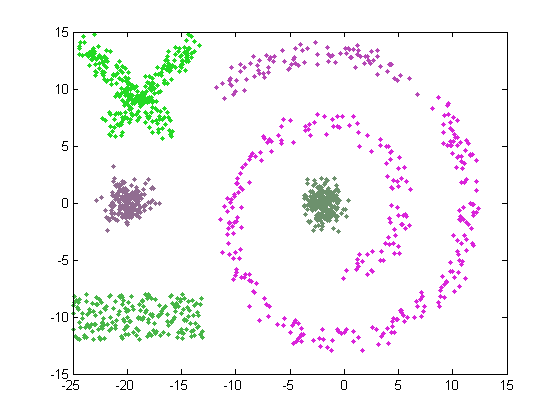
\includegraphics[scale=0.65]{fig/dbscan-non-noisy-data.png}
%   \caption{DBScan on non-noisy data where Minpts = 14 and Eps = 1.6}
%   \label{fig:dbscan-non-noisy-data}
% \end{center}
% \end{figure}
		
	\item (15 points) Use DbScan on the noisy data. Try different settings of parameter Minpts and Eps. Plot the best clustering result you think, and answer:
		\begin{itemize}
  			\item How the clustering result is changing when you increase Minpts ?
  			
  			\textbf{Answer:} The number of clusters decreases.
  			
			\item How the clustering result is changing when you increase Eps ?
			
			\textbf{Answer:} The number of clusters increases.
		\end{itemize}
		
		When the Minpts = 8 and Eps = 1.4, the clustering result looks pretty good. Figure \ref{fig:noisy-data} shows the plot of noisy data and Figure \ref{fig:dbscan-noisy-data} shows the clustering result using DBScan.
		
		
		\begin{figure}[!iht]
		\centering
 		 \subfigure[Noisy data]{
			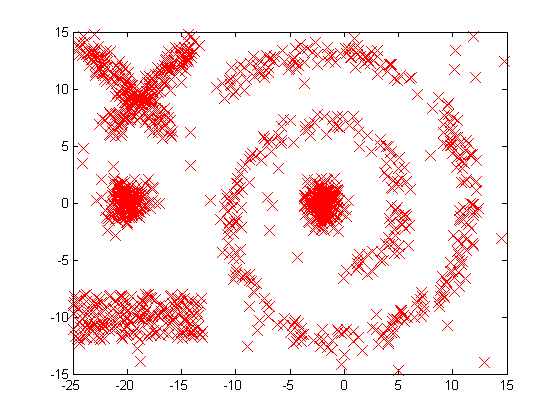
\includegraphics[scale=0.5]{fig/data2.png}
		    \label{fig:noisy-data}
		}
		\subfigure[DBScan on noisy data where Minpts = 8 and Eps = 1.4]{
			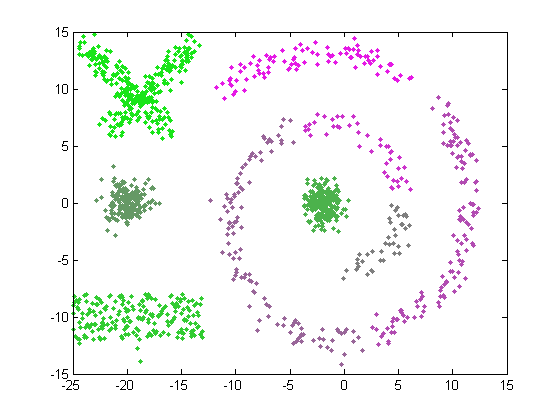
\includegraphics[scale=0.5]{fig/dbscan-noisy-data.png}
	    	\label{fig:dbscan-noisy-data}
		}
		\caption{DBScan on noisy data}
		\end{figure}
		
% 		
% \begin{figure}[!iht]
% \begin{center}
%   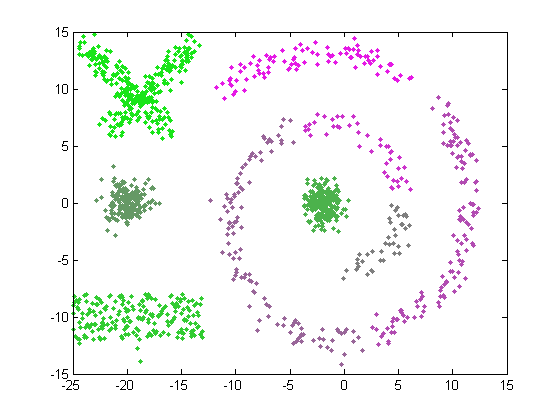
\includegraphics[scale=0.65]{fig/dbscan-noisy-data.png}
%   \caption{DBScan on noisy data where Minpts = 8 and Eps = 1.4}
%   \label{fig:dbscan-noisy-data}
% \end{center}
% \end{figure}
\end{enumerate}
\end{document}
